\documentclass{standalone}
\usepackage{tikz}
\begin{document}
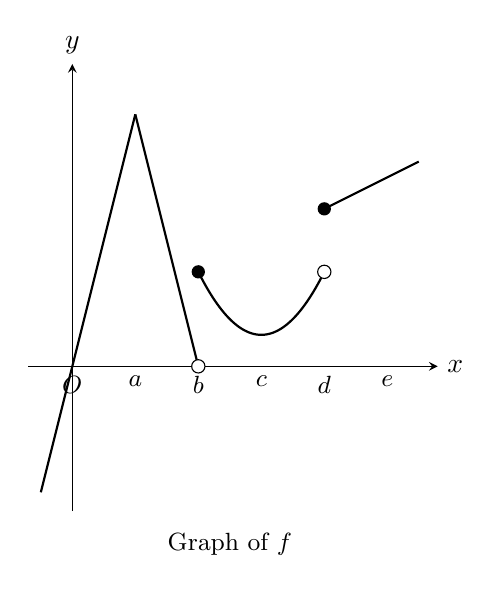
\begin{tikzpicture}[>=stealth, scale=0.8]
  % Axes
  \draw[->] (-0.7,0) -- (5.8,0) node[right] {$x$};
  \draw[->] (0,-2.3) -- (0,4.8) node[above] {$y$};

  \begin{scope}
    \clip (-0.7,-2.3) rectangle (5.8,4.7);
    % Left rise to corner: y=4x from x=-0.5 to x=1 (slope 4, through origin O)
    \draw[thick] (-0.5,-2) -- (1,4);
    % Right descent from corner to b: slope -4, open circle at (2,0)
    \draw[thick] (1,4) -- (2,0);
    % Smooth parabola (x-3)^2 + 0.5 from x=2 to x=4, open circle at (4,1.5)
    \draw[thick] plot[domain=2:4,samples=60] (\x,{(\x-3)*(\x-3)+0.5});
    % Continuation past d: from (4,2.5) to (5.5,3.25), slope 0.5
    \draw[thick] (4,2.5) -- (5.5,3.25);
  \end{scope}

  % Open circle at (2,0): f not continuous at b
  \draw[fill=white,draw=black] (2,0) circle (3pt);
  % Filled dot at (2,1.5): actual value of f at b
  \fill[black] (2,1.5) circle (3pt);
  % Open circle at (4,1.5): f not continuous at d
  \draw[fill=white,draw=black] (4,1.5) circle (3pt);
  % Filled dot at (4,2.5): actual value of f at d
  \fill[black] (4,2.5) circle (3pt);

  % x-axis labels: O, a, b, c, d, e
  \node[below,font=\small] at (0,0)  {$O$};
  \node[below,font=\small] at (1,0)  {$a$};
  \node[below,font=\small] at (2,0)  {$b$};
  \node[below,font=\small] at (3,0)  {$c$};
  \node[below,font=\small] at (4,0)  {$d$};
  \node[below,font=\small] at (5,0)  {$e$};

  % Title below
  \node[below,font=\small] at (2.5,-2.5) {Graph of $f$};
\end{tikzpicture}
\end{document}
